% 图 6.2 液相无序点云 (T>Tc) 与固相规则点阵 (T<Tc)
\documentclass[tikz,border=5pt]{standalone}
\usetikzlibrary{arrows.meta}
\usepackage{amsmath}
\usepackage{bm}
\usepackage{fontspec}
\setmainfont{Times New Roman}
\begin{document}
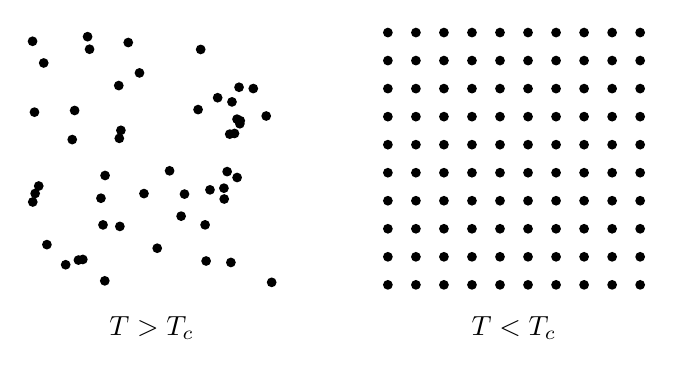
\begin{tikzpicture}[line width=0.8pt,>=Stealth]
\pgfmathsetseed{20260602}
% ---- left: disordered liquid, ~50 random dots ----
\begin{scope}[shift={(0,0)}]
  \foreach \i in {1,...,50}{
    \pgfmathsetmacro\x{1.6+1.6*rand}
    \pgfmathsetmacro\y{1.6+1.6*rand}
    \fill (\x,\y) circle (0.062);
  }
  \node at (1.6,-0.55) {$T>T_c$};
\end{scope}
% ---- right: ordered 10x10 lattice ----
\begin{scope}[shift={(4.6,0)}]
  \foreach \i in {0,...,9}{\foreach \j in {0,...,9}{
    \fill ({\i*0.356},{\j*0.356}) circle (0.062);
  }}
  \node at (1.6,-0.55) {$T<T_c$};
\end{scope}
\end{tikzpicture}
\end{document}
